% !TeX root = ../main.tex
% -*- coding: utf-8 -*-

\chapter{实验设计与分析}
在本章中我们将对CLML算法展开一系列实验,希望通过对比,得到CLML算法的准确率、鲁棒性等指标,以及它在实际应用中的表现,并试图从数据集的特点上探究影响算法性能的因素。 


\section{实验数据与参数设置}
\subsection{评价指标}
在分类问题中,我们经常会计算出样本在每个类别下的概率,这样做可通过设置阈值来满足对模型的不同需求。
例如,(在二分类问题中)当阈值设为0.5时,所有输出概率在[0, 0.49]范围内的样本将被标记为负类(Negative),
在[0.5, 1.0]的样本便被标记为正类(Positive)。根据样本的真实类别与算法预测类别的组合可将样本划分为四类,
分别为:真正例(True Positive,TP)、假正例(False Positive,FP)、真反例(True Negative,TN)、假反例(False Negative,FN)。
据此,我们可得到表\ref{experiments:table:mix_matrix}中的“混淆矩阵”,它表明样本是否被错误分类,是评估分类算法的基础。

\begin{center}
    \tablecaption{混淆矩阵}
    \begin{tabular}{|c|c|c|} \hline
        \multirow{2}{*}{真实情况} & \multicolumn{2}{c|}{预测结果} \\ \cline{2-3}
                                & 正例  & 反例  \\ \hline
        正例                     & 真正例(TN)   & 假反例(FN) \\ \hline
        反例                     & 假正例(FP)   & 真反例(TN) \\ \hline
    \end{tabular}
    \label{experiments:table:mix_matrix}
\end{center}

\begin{enumerate}
    \item ROC:ROC曲线全名为Receiver Operating Characteristic curve,即“受试者工作曲线”,是衡量二分类算法的一个常用指标。
    曲线画出了当阈值在[0.0, 1.0]范围内变化时,模型真正例率(True Positive Rate,TPR)和假正例率(False Negative Rate,FNR)的变化情况。
    TPR和FNR分别定义为:
    \[ TPR = \frac{True Positives}{True Positives + False Negatives} \]
    \[ FPR = \frac{False Positives}{False Positives + True Negatives} \]
    ROC在二分类算法中经常被使用的原因为:首先,可在ROC曲线图中直观地对比不同的算法;其次,ROC曲线下的面积(AUC)可作为模型性能的总结[26]。
    \item AUC:AUC(Area Under Curve of ROC)[26]是评估模型预测结果质量时最常用的一个指标。
    每个样本都有一个概率,在计算时首先分别从正例和负例集合中随机选取一条链接,然后比较两者的预测概率,共重复n次。
    若在这n次采样中,有n次前者概率大于后者,有n次两者相等,则模型的AUC为:
    \[AUC=\frac{n^{'}+0.5n^{''}}{n}\]
    显然,AUC越高代表模型的预测结果越好。从对公式的介绍中也可看出,最好情况下,所有已存在的链接上预测的值应均大于不存在的链接,此时AUC的值为1;随机分类器的AUC应接近0.5。
    \item AUC20:由于我们的算法更加侧重于预测出的高概率链接,因此我们限制预测出的FP数量要小于等于20,并将该结果也作为一个评价指标。
    \item AUPR: AUPR[33] 全称为Area Under curve of Precision-Recall,其中查准率P(precision)和查全率R(recall)分别定义为:
    \[P=\frac{TP}{TP+FP}\] \[R=\frac{TP}{TP+FN}\]
    显然查准率和查全率是一对相互矛盾的度量(P高时R往往偏低,反之亦然)。
    类似于画ROC曲线的方式,PR曲线描述了当阈值变化时查准率和查全率的关系,曲线下方的面积(AUPR)提供了对正确预测出正类和负类比例的量化性评估[10]。
    由于在链接预测问题中,负类样本数量往往远多于正类样本,而AUPR又更多地惩罚FP类的样本,因此AUPR是一个比AUC更有价值的测量指标[10].
\end{enumerate}


\subsection{数据集介绍和交叉验证实验}
\label{experiments:sec:db_cv}
实验时我们从四个完全不同的领域挑选出了四个数据集,分别为:
\begin{enumerate}
    \item Douban Movie数据集,Douban Movie是国内一个知名的影评网站(加上脚注),用户可在网站上对任意电影从1至5打分;
    此外,用户还可添加好友,进行一定程度的社交。又因为不同电影可以根据类别、演员、语种甚至上映日期分类,
    故我们可选定一些特征将电影分类,规定某一类中的电影是彼此相似的。通过在该网站爬取上述信息,
    我们便可构建出用户-用户关联矩阵$D$、用户-电影关联矩阵$R$以及电影-电影关联矩阵$T$。
    \item Yelp数据集,Yelp是国外一个很常用的商户点评网站,用户可在其上对到访过的商户打分、评论以供后人参考。
    使用类似处理Douban数据集的方法,我们同样可以获得$D$、$R$、$T$矩阵。
    \item NIPS合作数据集包含了在特定科研领域中发表的论文与其作者,以及最具特点的:不同作者间相互合作的关系。
    例如,若作者A和作者B共同参与发表了一篇论文,则可认为A和B进行了一次合作。该数据集也因此受到了来自不同领域学者的广泛关注。
    \item DDI数据集,如第一章所述,DDI表示不同药物在临床共同使用时是否会发生相互作用。
    与之类似,DPI(Drug-Protein Interaction)网络代表药物对与靶蛋白之间的关系(许多药物都是通过影响特定蛋白质的合成来治疗疾病的)、
    PPI(Protein-Protein Interaction)代表蛋白质与蛋白质间的作用(许多疾病、基因表型往往是多种蛋白共同作用的结果)。
    Drugbank是一个权威的生物医学信息网站,其每一两个月就会统计各文献、临床报告中发现的新的DDI、DPI和PPI,
    整理后发布到其官网上供学者研究。
\end{enumerate}


需要指出,原始数据包含许多其它信息且格式不统一,我们使用的均是由[25]提供的清洗后的数据。


表\ref{experiments:table:simple_stats}初步统计了从四个数据集中构建的$D$、$R$、$T$矩阵的特点。
从表格中可以粗略看出Douban数据集的样本数最多(A、B数量均高于其他数据集),
但A-A关联矩阵却较为稀疏;相反,DDI数据集包含的样本数量很少(采样成本远高于其他三个),
但A-A矩阵有近四分之一的非零元素;Yelp数据集中不仅样本数量大,且矩阵也含有相对较多的非零元素。


为进一步帮助理解数据集的特点,我们又分析了每个数据集中节点度数的分布(图\ref{experiments:fig:node_distribution}),
并统计了每个数据集的聚类系数、平均度数、平均最短路径等分析复杂网络常用的统计指标,见表\ref{experiments:table:simple_stats}。


\begin{center}
    \tablecaption{对四个数据集的初步统计数据}
    \begin{tabular}{@{\extracolsep{\fill}}c|cccc}\hline
        数据集        & Douban & Yelp & NIPS & DDI \\ \hline
        关系(A-B)   & 用户-电影 & 用户-商家 & 作者-出版物 & 药物-靶蛋白 \\
        A的数量       & 13367   & 16239  & 2865  &  758  \\
        B的数量       & 12677   & 14284  & 2484  &  473  \\
        A-A的数量     & 4085    & 158590 & 63178 & 11852 \\
        A-B的数量     & 168278  & 198397 & 5879  & 2296  \\ \hline
    \end{tabular}
    \label{experiments:table:simple_stats}
\end{center}

\begin{figure}[]
    \centering
    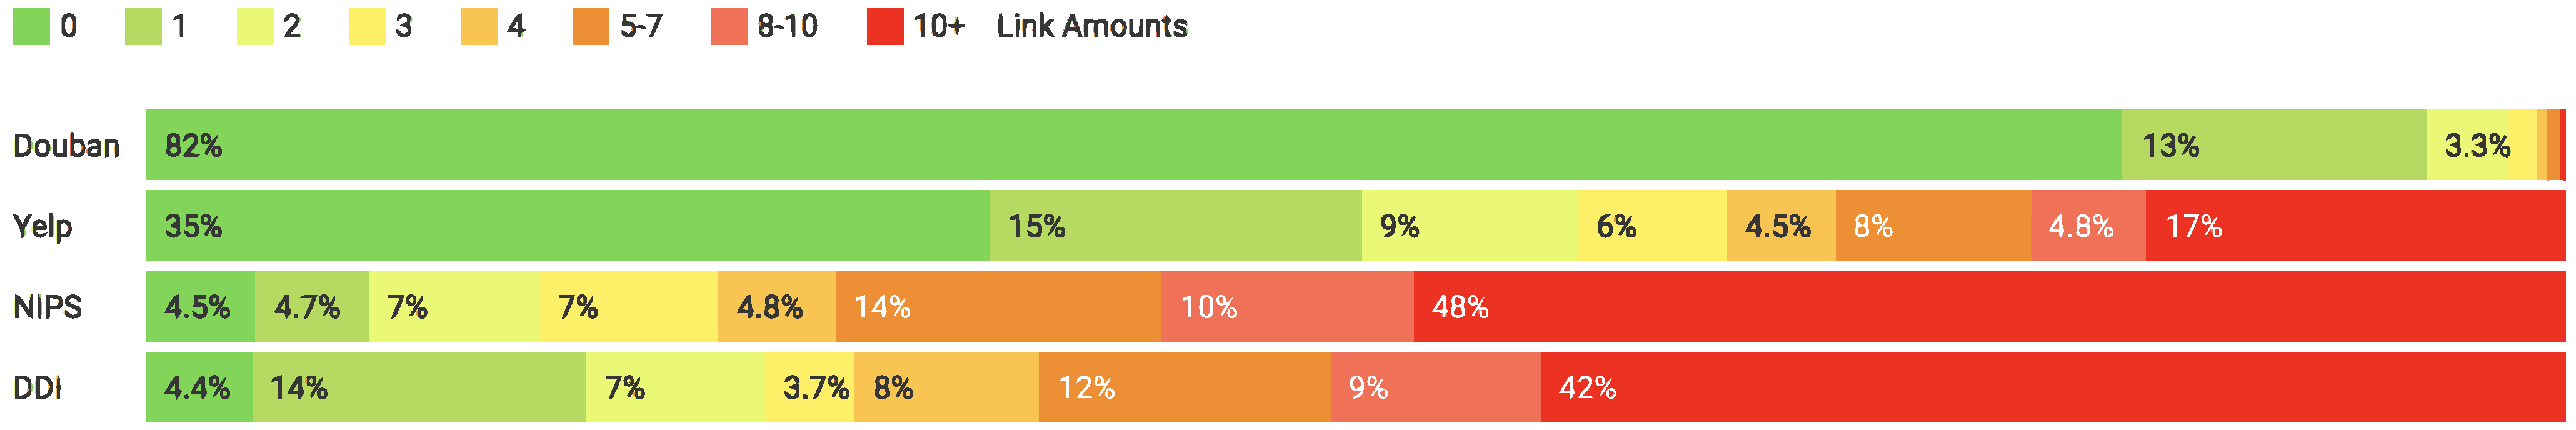
\includegraphics[width=0.98\linewidth, height=3cm]{node_distribution.pdf}
    \caption{各数据集节点度数分布}
    \label{experiments:fig:node_distribution}
\end{figure}


\begin{center}
    \tablecaption{各数据集拓扑结构的详细信息}
        \begin{tabular}{c|cccc}\hline
            数据集          & Douban & Yelp & NIPS & DDI \\ \hline
            聚类系数        & 0.017 & 0.226 & 0.609 & 0.164 \\
            网络密度       & 0.001   & 0.001  & 0.009  &  0.023  \\
            网络直径     & 29   & 11  & 11  &  7  \\
            最短路径     & 4309882(43\%)    & 1071952414(95\%) & 5820682(84\%) & 524900(100\%) \\
            平均近邻数     & 1.948  & 14.990 & 23.048  & 16.348  \\ \hline
        \end{tabular}
        \label{experiments:table:simple_stats}
\end{center}

实验时,我们随机选取80\%的数据作为训练集,记录并删掉剩余的20\%数据作为测试集,然后用在训练集上的预测结果与测试集做对比。
模型训练时使用5*10折交叉验证,即我们将训练集随机划分为10份,每轮依次使用其中的1份作为验证集,剩余的9份作为训练集,
重复5次取平均数作为本次模型的结果,代码3.1为交叉验证的关键代码:



\begin{lstlisting}[caption={交叉验证的关键代码},language=Matlab]
    function [ result ] = CrossValidationOf-
    DualManifoldWithLowRank(R, D, W1, T, W2, alpha, beta, gamma,
     maxIterator, fold,density)
    % m 是矩阵 R 的行数
    [m, ~] = size(R); 
    % base 是每折的样例数
    base = floor(m / fold); 
    % result 保存计算出的每折的平均 AUC 和 AUPR
    result = zeros(fold, 2); 
    
    % iterate process 具体的迭代过程
    for i = 1:fold % 分别对每一折进行计算
        lastNum = base * i; % 每一折的末尾行号
        beginNum = lastNum - base + 1; % 每一折的开始行号
        
        trainData = D; % 同时抹去 D 中这一折的行和列,
        trainData(beginNum:lastNum, :) = 0; % 作为训练集
        trainData(:, beginNum:lastNum) = 0;       
        T = eraseData(T,density);
        % 学习得到预测的 D = |D| + |D'|;
        predictData = abs(DualManifoldWith-
        LowRank(R, trainData, W1, T, W2, alpha, beta,
         gamma, maxIterator));
        predictData = predictData + predictData';
       .......
        % 一折结束
    end
    result = mean(result, 1); % 对最后的结果求平均
    end
\end{lstlisting}

\subsection{对比算法}
在\ref{intro:sec:study}中我们提到,链接预测算法大致分为三类,因此我们从这三类中分别挑选出了一些比较有代表性的算法。
我们在基于相似度的算法中选取了CN、AA、NSI算法;
在基于路径的算法中选取了LP、MCLP;
在矩阵分解算法中选取了MF、MRMF算法;
除此之外,我们称未引入协同学习时的算法为LML,将其也作为一个对比算法来一并研究协同学习在算法中的作用。

\section{实验设计与分析}
\subsection{算法性能结果}
我们分别使用四个数据集对CLML算法和其它对比算法进行测试,在选取了最佳参数后,
我们得到了表\ref{experiments:table:auc20}~\ref{experiments:table:aupr}中的数据,
表中加粗的结果代表每个数据集下取得的最大值。从中我们可以看出,基于线性流形学习的方法,无论是LML还是CLML都较大部分算法而言有明显提升;
而使用了两个线性流形进行协同学习的CLML与LML相比更是在各项指标中均有显著提升,在AUPR上甚至提升了近50\%。
注意到,MRMF算法在Yelp数据集中的AUC20要优于LML和CLML,但该算法的AUC和AUPR却均低于我们的算法。
因此我们可以初步得出结论:CLML算法的性能优于其它对比算法。


此外,从各算法的AUC值可以看出,基于特征提取(feature extraction)、标签传播(label propagation)的算法在链接预测问题上并不适用,
AUC值接近甚至低于0.5,因为这些算法并没有利用辅助信息也没有考虑到数据的结构特点。
与之相反,CLML不仅利用了数据集中的辅助信息,也考虑了数据的流形结构和低秩特性,这也是CLML在此类数据集上的优点。 

\begin{center}
    \tablecaption{各算法的AUC20值对比}
    \begin{tabular}{c|cccc} \hline
        算法 & Douban & Yelp & NIPS & DDI \\ \hline
        CN  & 0.0213 & 0.0568 & 0.0193 & 0.0161 \\
        AA  & 0.0290 & 0.0282 & 0.0173 & 0.0251 \\
        NSI & 0.1725 & 0.2088 & 0.1751 & 0.2879 \\
        LP  & 0.0569 & 0.2447 & 0.1066 & 0.3643 \\
        MCLP& 0.1528 & 0.1321 & 0.0511 & 0.0837 \\
        MF  & 0.1949 & 0.2895 & 0.1722 & 0.1760 \\
        MRMF& 0.1574 & \bfseries 0.3545 & 0.1481 & 0.3679 \\ \hline
        LML & 0.1349 & 0.0843 & 0.1990 & 0.1584 \\
        CLML& \bfseries 0.3014 & 0.2070 & \bfseries 0.2281 & \bfseries 0.5436 \\ \hline
    \end{tabular}
    \label{experiments:table:auc20}
\end{center}


\begin{center}
    \tablecaption{各算法的AUC值对比}
    \begin{tabular}{c|cccc} \hline
        算法&	Douban & Yelp & NIPS & DDI \\ \hline
        CN  & 0.5186 & 0.5804 & 0.5038 & 0.5121 \\
        AA  & 0.5248 & 0.5489 & 0.5057 & 0.5388 \\
        NSI & 0.6474 & 0.6731 & 0.6097 & 0.6437 \\
        LP	& 0.5520 & 0.6969 & 0.4621 & 0.7136 \\
        MCLP& 0.6904 & 0.7269 & 0.6357 & 0.7322 \\
        MF  & 0.6710 & 0.6884 & 0.5895 & 0.6503 \\
        MRMF& 0.6658 & 0.7475 & 0.6243 & 0.8186 \\ \hline
        LML & 0.6551 & 0.6358 & 0.6210 & 0.8040 \\
        CLML& \bfseries 0.7203 & \bfseries 0.7808 & \bfseries 0.6438 & \bfseries 0.8297 \\ \hline
    \end{tabular}
    \label{experiments:table:auc}
\end{center}

\begin{center}
    \tablecaption{各算法的AUPR值对比} 
    \begin{tabular}{c|cccc} \hline
        算法 &	Douban & Yelp & NIPS & DDI \\ \hline
        CN  & 0.0115 & 0.0229 & 0.0171 & 0.0292 \\
        AA  & 0.0085 & 0.0141 & 0.0170 & 0.0322 \\
        NSI & 0.0870 & 0.1273 & 0.1160 & 0.1506 \\
        LP	& 0.0285 & 0.1341 & 0.0927 & 0.3490 \\
        MCLP& 0.0519 & 0.0750 & 0.0398 & 0.0795 \\
        MF  & 0.1043 & 0.2266 & 0.1137 & 0.0814 \\
        MRMF& 0.0744 & 0.2548 & 0.1269 & 0.3679 \\ \hline
        LML & 0.1622 & 0.1370 & 0.1717 & 0.3287 \\
        CLML& \bfseries 0.2488 & \bfseries 0.2642 & \bfseries 0.1751 & \bfseries 0.3917 \\ \hline
    \end{tabular}
    \label{experiments:table:aupr}
\end{center}

\subsection{后续检验}

通过观察数据初步得出了CLML优于其它算法的结论,但仅凭比较测试结果的大小还远不足以下最终定论,主要有以下几个原因:
第一,实验数据是在测试集上的结果,而我们希望比较的是模型间的泛化性能,二者有一定的差别;
第二,实验数据和测试集的选取有很大关系,即便使用同样大小的测试集,得出的结果也会因测试数据不同而不同,也可以说实验数据带有一定的随机性;
第三,无论CLML还是其它比较算法,在调参、优化过程中本身就有一定的随机性,即便参数设置相同、数据集相同,每次得到的结果也会有所不同。
因此,想要得出CLML优于其它算法这一结论,我们还需要做比较检验,以获得统计意义上的结论。
为要比较多个算法在多个数据集上的性能,我们引入了基于算法排序的弗里德曼检验(Friedman test)
再这之后又使用Nemenyi后续检验(Nemenyi post-hoc test)进一步区分了各算法。


令$N$表示数据集个数,$k$表示算法个数,$r_i$表示第$i$个算法的平均排名,则$r_i$的平均值和方差分别为$(k+1)/2$和$(k^2-1)/12$。变量

\begin{equation}
    \tau_{\chi^2} =\frac{k-1}{k}\cdot\frac{12N}{k^2-1}\sum_{i=1}^k(r_i-\frac{k+1}{2})^2 =\frac{12N}{k(k+1)}(\sum_{i=1}^kr_i^2-\frac{k(k+1)^2}{4})
    \label{experiments:formula:tau}
\end{equation}

在$k$和$N$都较大时,$\tau_{\chi^2}$服从自由度为$k-1$的卡方分布。不过目前在做弗里德曼检验时通常使用的是变量:

\begin{equation}
    \tau_F=\frac{(N-1)\tau_{\chi^2}}{N(k-1)-\tau_{\chi^2}} 
    \label{experiments:formula:tauF}
\end{equation}
    
其中$\tau_{\chi^2}$的值由式(\ref{experiments:formula:tau})得到,$\tau_F$服从自由度为$k-1$的F分布,表\ref{experiments:table:F_test}给出了F检验的常用临界值。

\begin{center}
    \tablecaption{F检验在α=0.1时常用的临界值}
    \begin{tabular}{|c|ccccccccc|} \hline
        \multirow{2}{*}{数据集个数N} & \multicolumn{9}{c|}{算法个数} \\ \cline{2-10}
         & 2 & 3 & 4 & 5 & 6 & 7 & 8 & 9 & 10 \\ \hline
        4 & 5.538 & 3.463 & 2.813 & 2.480 & 2.273 & 2.130 & 2.023 & 1.940 & 1.874 \\
        5 & 4.545 & 3.113 & 2.606 & 2.333 & 2.158 & 2.035 & 1.943 & 1.870 & 1.811 \\
        8 & 3.589 & 2.726 & 2.365 & 2.157 & 2.019 & 1.919 & 1.843 & 1.782 & 1.733 \\
        10 & 3.360 & 2.624 & 2.299 & 2.108 & 1.980 & 1.886 & 1.814 & 1.757 & 1.710 \\
        15 & 3.102 & 2.503 & 2.219 & 2.048 & 1.931 & 1.845 & 1.779 & 1.726 & 1.682 \\
        20 & 2.990 & 2.448 & 2.182 & 2.020 & 1.909 & 1.826 & 1.762 & 1.711 & 1.668 \\ \hline
    \end{tabular}
    \label{experiments:table:F_test}
\end{center}


\begin{center}
    \tablecaption{算法结果的排名统计}
    \begin{tabular}{|c|ccccccccc|} \hline
           & CLML & LML & CN & AA & NSI & LP & MCLP & MCRI & MRMF \\ \hline
        Douban & 1 & 5 & 9 & 8 & 6 & 7 & 2 & 3 & 4 \\
        Yelp & 1 & 7 & 8 & 9 & 6 & 4 & 3 & 5 & 2 \\
        NIPS & 1 & 4 & 8 & 7 & 5 & 9 & 2 & 6 & 3 \\
        DDI  & 1 & 3 & 9 & 8 & 7 & 5 & 4 & 6 & 2 \\ \hline
        平均 & 1 & 4.75 & 8.5 & 8 & 6 & 6.25 & 2.75 & 5 & 2.75 \\ \hline
    \end{tabular}
    \label{experiments:table:rank}
\end{center}

为计算上述变量的值,我们以算法的AUC值为例,计算了所有算法在不同数据集中AUC值的排名,见表\ref{experiments:table:rank}。




设$H_0$假设为“所有算法的性能相同”,显著度$\alpha=0.1$。则在本题中$N=2$,$k=9$,$r_i$的均值为$(k+1)/2=(9+1)/2=5$
(不考虑平分序值的情况),方差为$(k^2-1)/12=(9^2-1)/12=20/3$,代入式(\ref{experiments:formula:tauF})中得到$\tau_F\approx{15.01}$,
对比表\ref{experiments:table:F_test}后不难发现,$\tau_F$大于F检验临界值1.940,因此我们拒绝$H_0$,即认为“算法的性能有差异”。


得到上述结论后,我们还想进一步比较各算法的具体差异,为此我们又在这之上引入了Nemenyi后续检验。
Nemenyi后续检验计算出平均排名差别的临界值域:

\begin{equation}
    CD=q_{\alpha}\sqrt{\frac{k(k+1)}{6N}}
    \label{experiments:formula:CD}
\end{equation}


当$\alpha=0.1$,$k=9$时Nemenyi检验常用的$q_{\alpha}$值为2.585,代入式(\ref{experiments:formula:CD})中计算出临界值域$CD\approx4.8$。
图\ref{experiments:fig:post_hoc}用弗里德曼检验图直观地展示了上述结果,其中:横轴代表排名,纵轴代表每个算法,图中横线长度代表临界值域CD(取CD=5),
每条横线中间的点表示各算法的平均排名。若两横线间有重叠区域则说明两算法无显著差异,若没有重叠区域则显然左边的算法性能要优于右边的算法。
从图中我们可以发现,CLML与所有基于节点或路径的算法有着显著差异(排名差异大于临界值域);
而和所有基于矩阵分解的算法相比,虽然CLML的性能更优,但差异却并不显著。

\begin{figure}[]
    \centering
    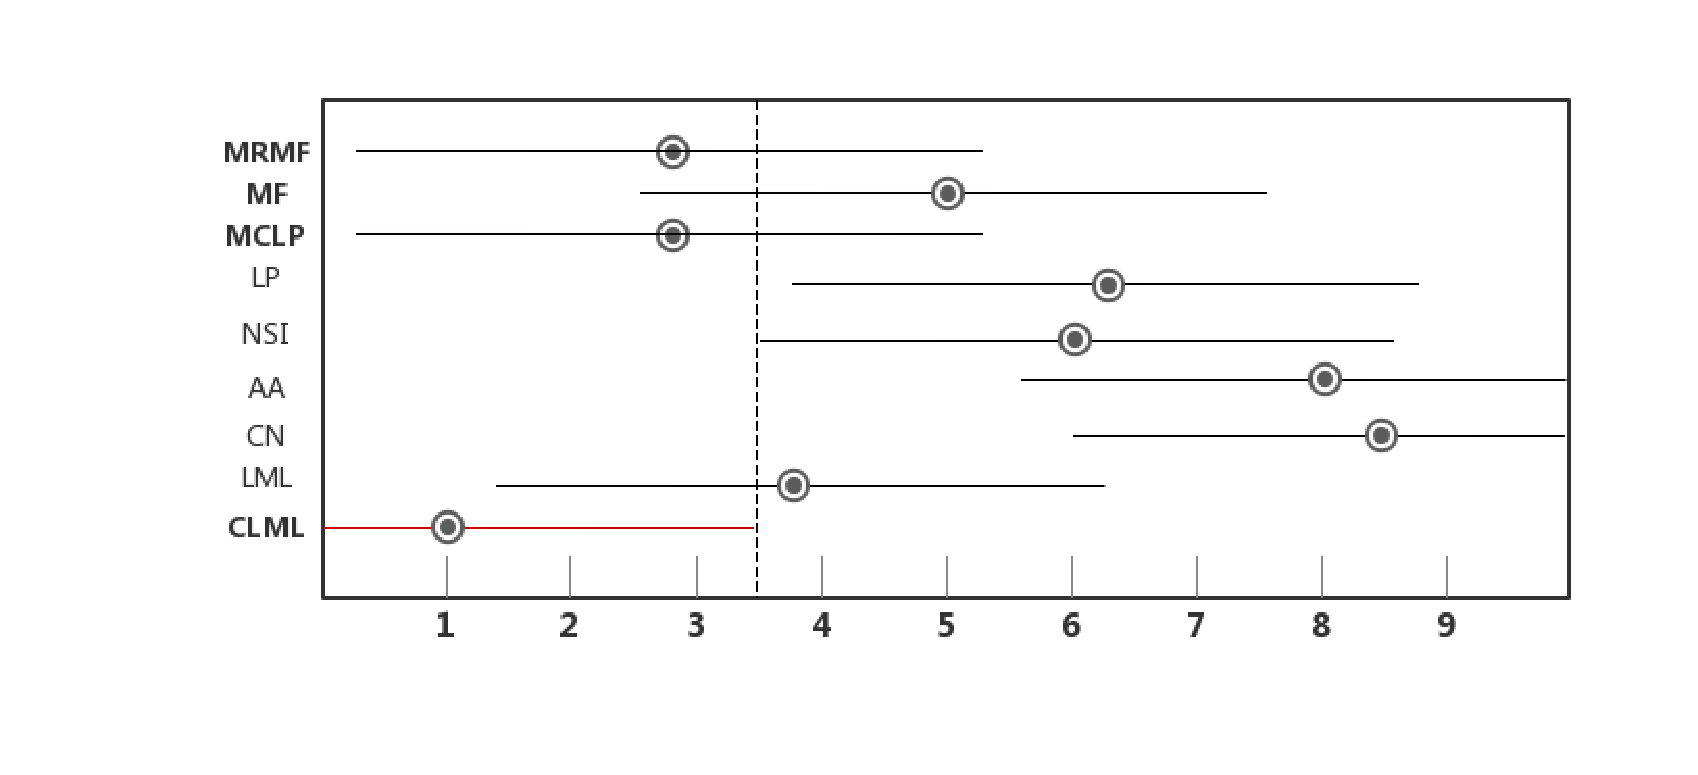
\includegraphics[width=0.9\linewidth]{post_hoc.pdf}
    \caption{弗里德曼检验图}
    \label{experiments:fig:post_hoc}
\end{figure}


在得到了算法在准确率相关的性能后,我们接着想到:算法的鲁棒性如何呢?
因为在概述中也提到过,要做链接预测的原因之一就是缺少足够的数据,如果我们的算法仅在数据丰富的情况下才能做出良好预测,那显然适用范围很窄。
在\ref{method:sec:collaborative}中我们指出,通过使用协同学习可以使数据不断富化从而很好地克服数据稀疏的问题,那么接下来我们将从实验的角度验证这一结论。


\subsection{算法鲁棒性实验}
为了验证算法鲁棒性,我们使用了[9][13][26]中的方法:
将所有矩阵(D、R、T矩阵)均随机删除同等程度的数据,再依次所有算法对其做预测得到删减数据后的结果,重复上述过程N次,每次删减不同程度的数据。
本次实验我们依次保留了80\%、60\%、40\%和20\%的数据,得到了如图\ref{experiments:fig:robust}的实验结果,其中横轴代表保留数据的比例,纵轴代表算法的AUC值。


\begin{figure}
    \centering
    \subfigure[DDI数据集]{
      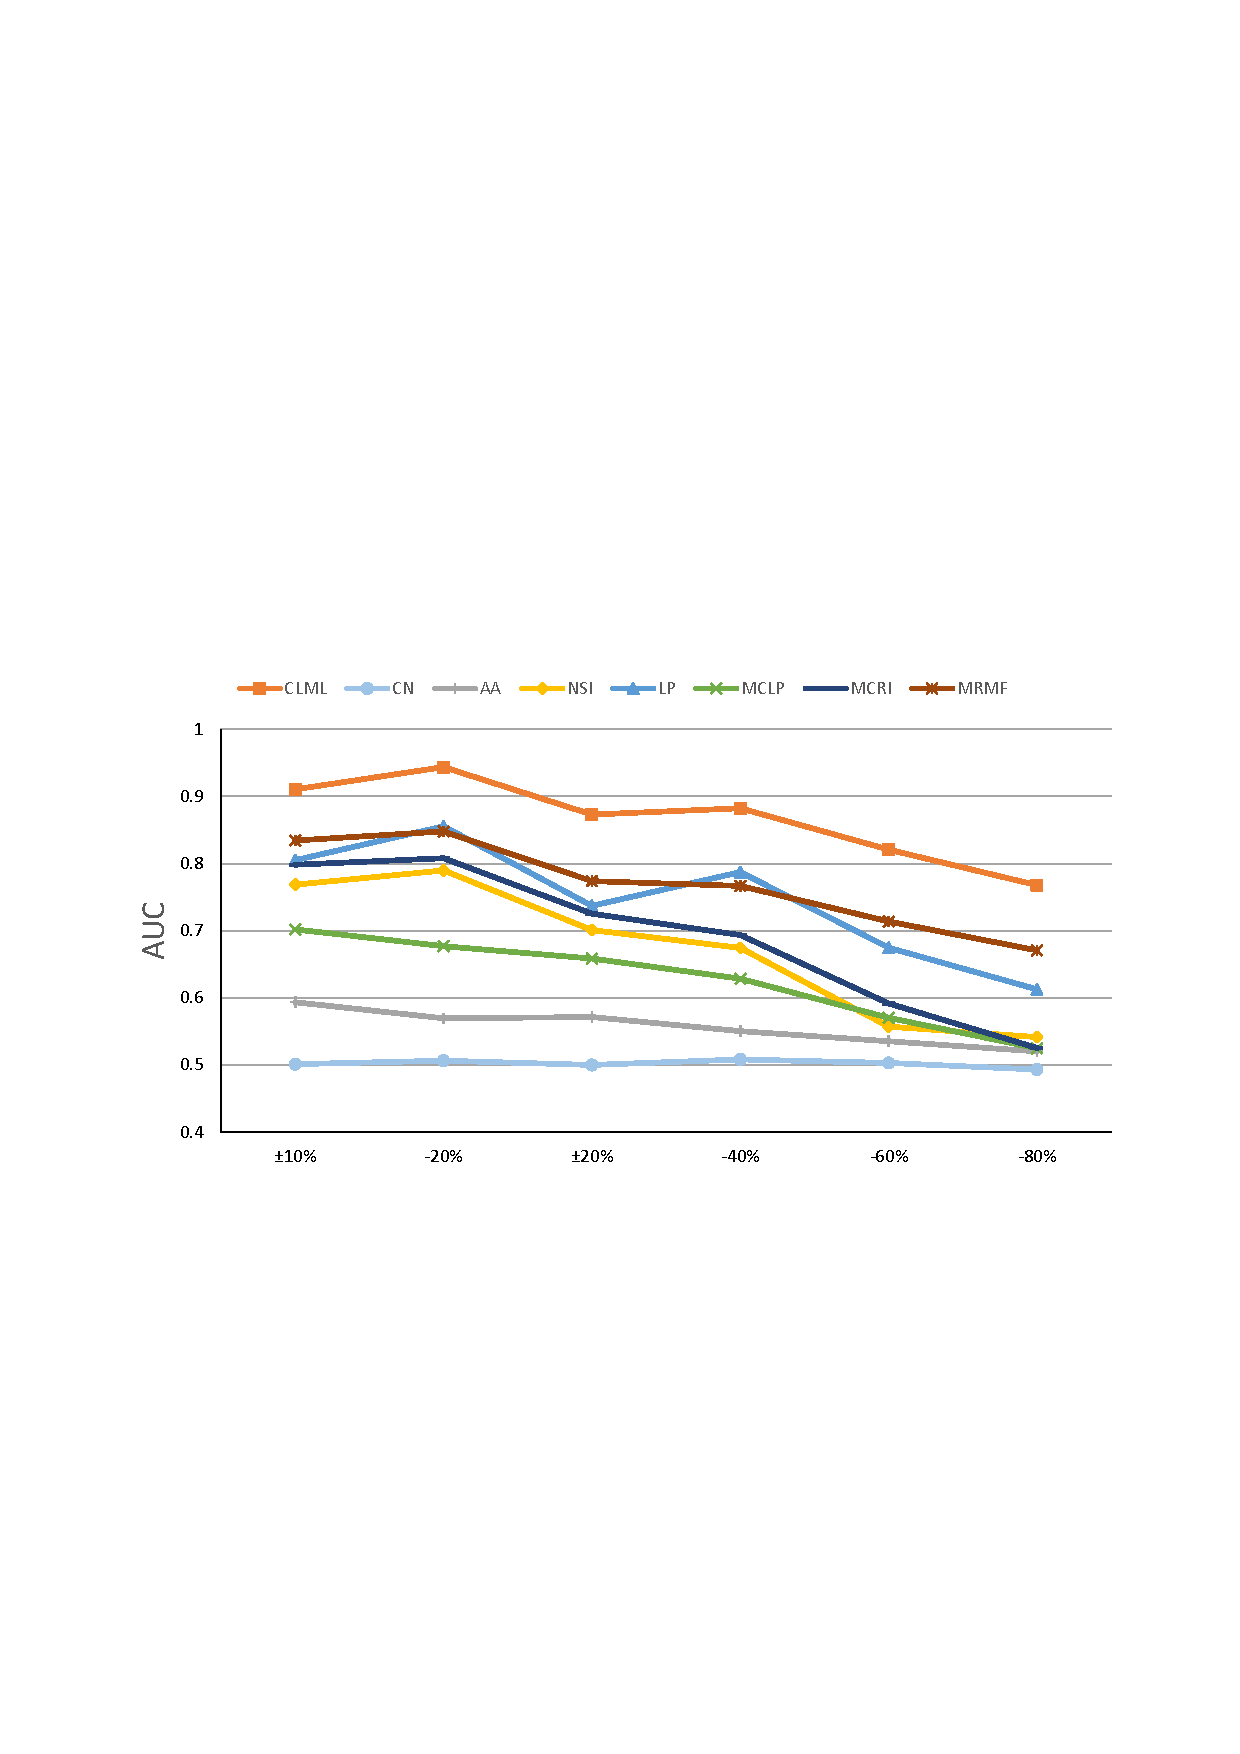
\includegraphics[width=0.45\linewidth]{AUC_DDI.pdf}
    }
    \subfigure[Yelp数据集]{
    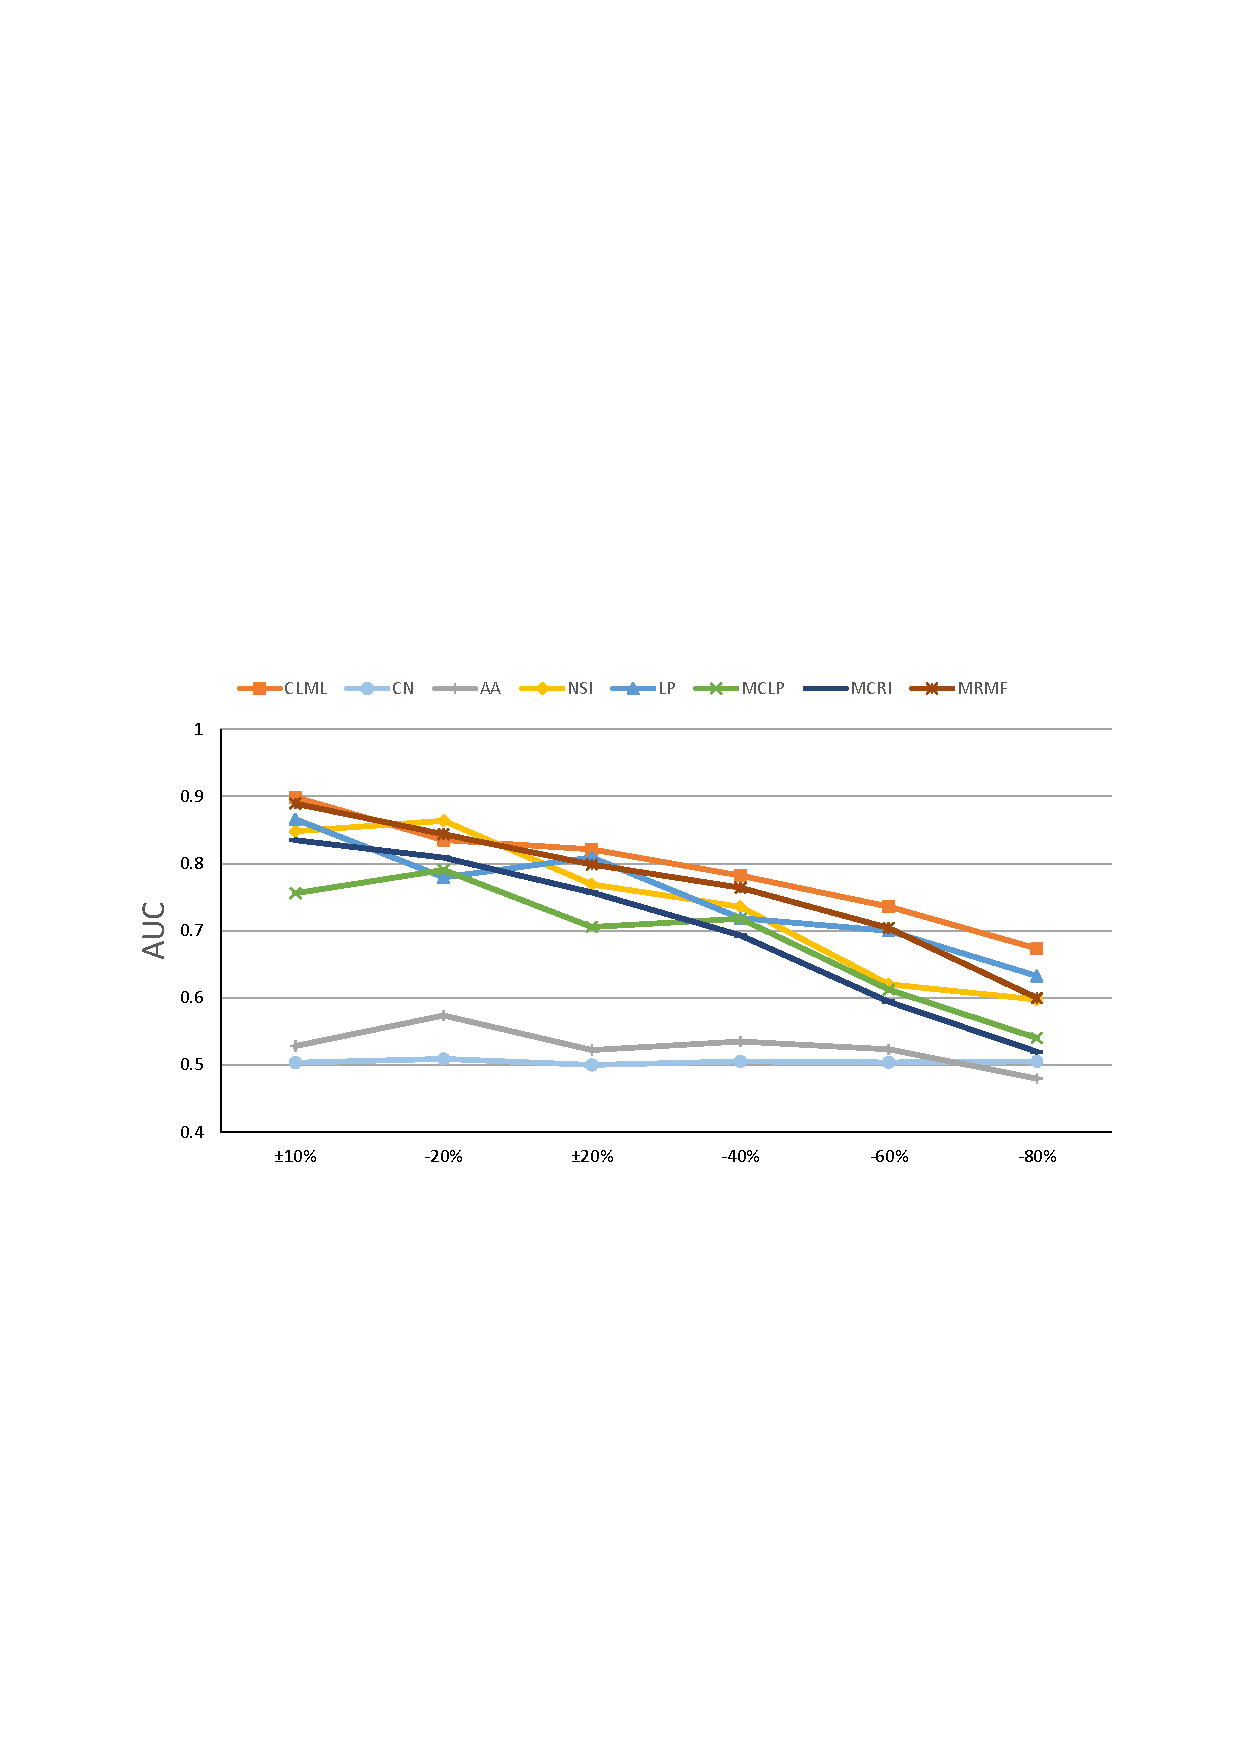
\includegraphics[width=0.45\linewidth]{AUC_Yelp.pdf}
    }
    \subfigure[Douban数据集]{
      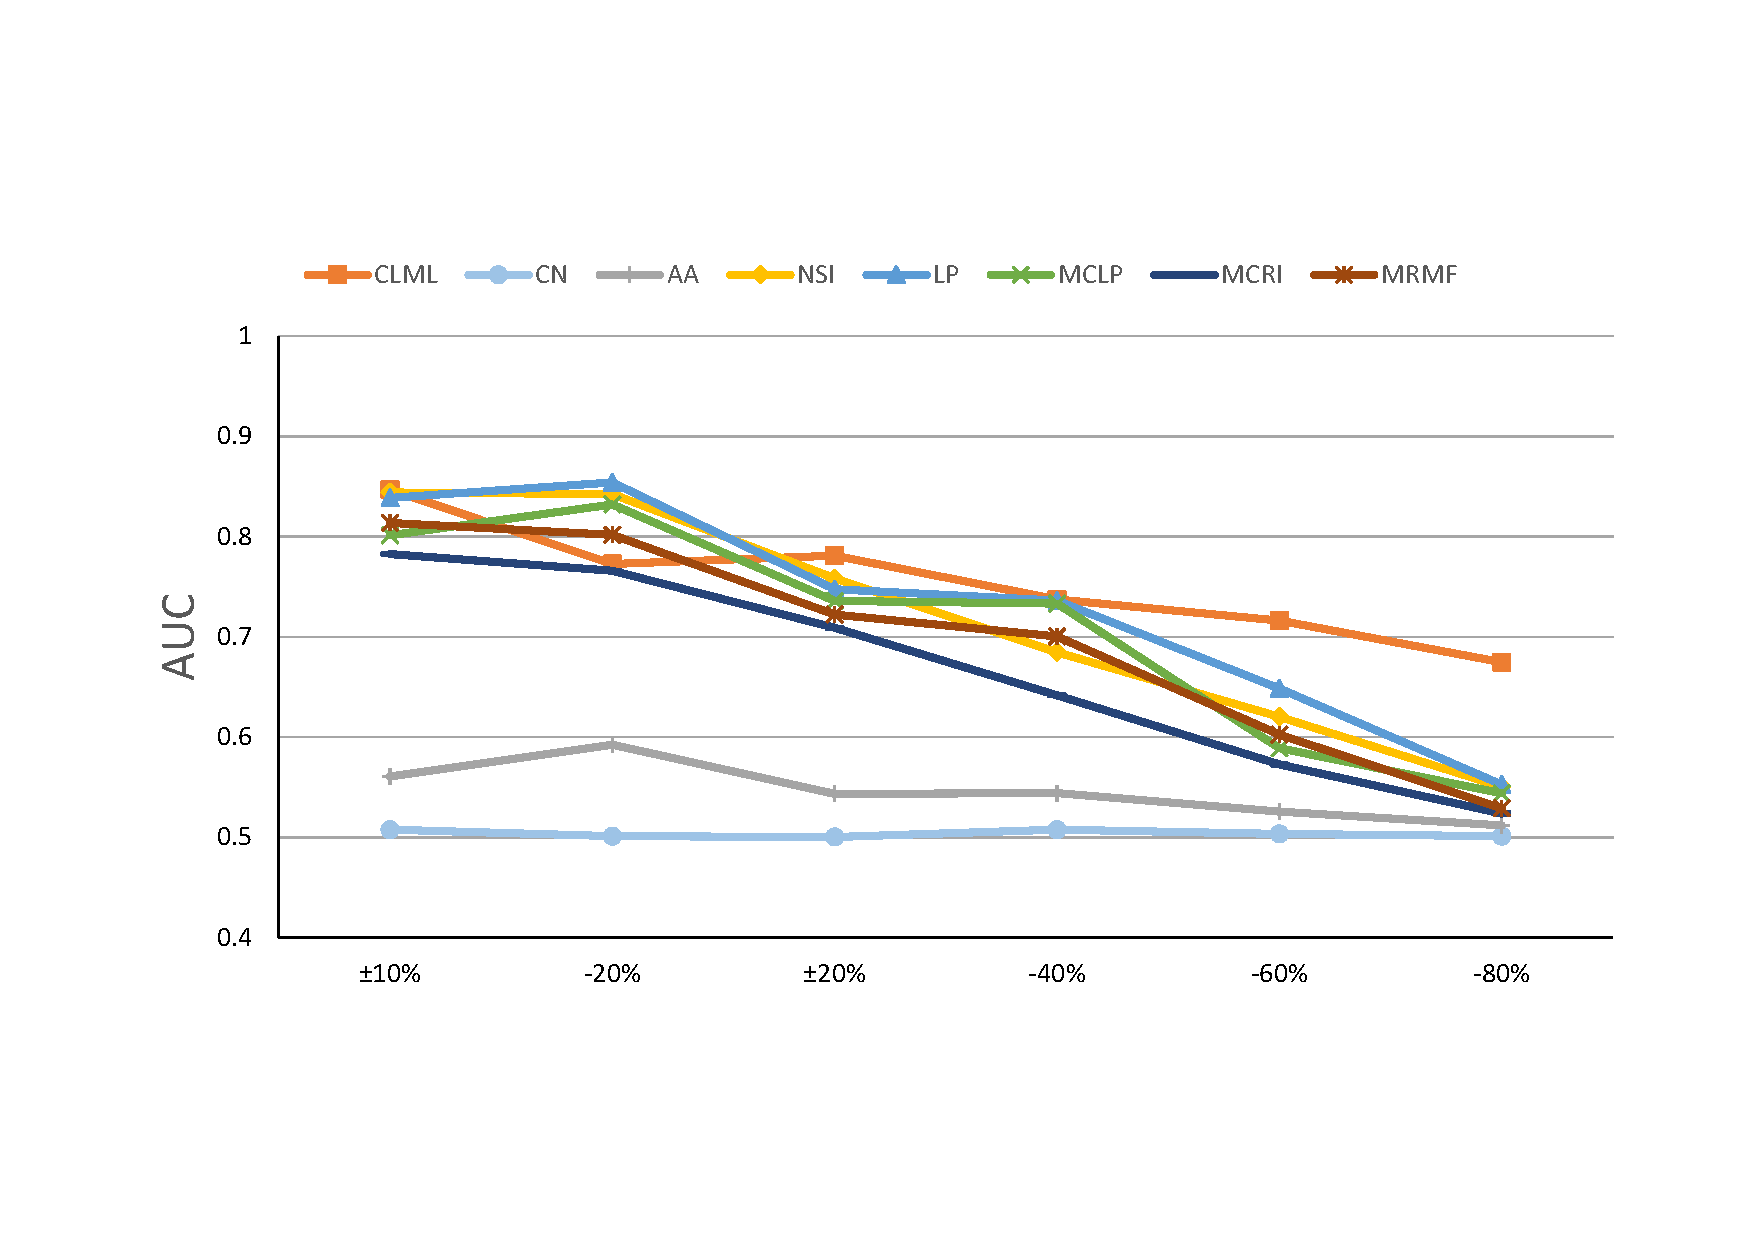
\includegraphics[width=0.45\linewidth]{AUC_Douban.pdf}
    }
    \subfigure[NIPS数据集]{
    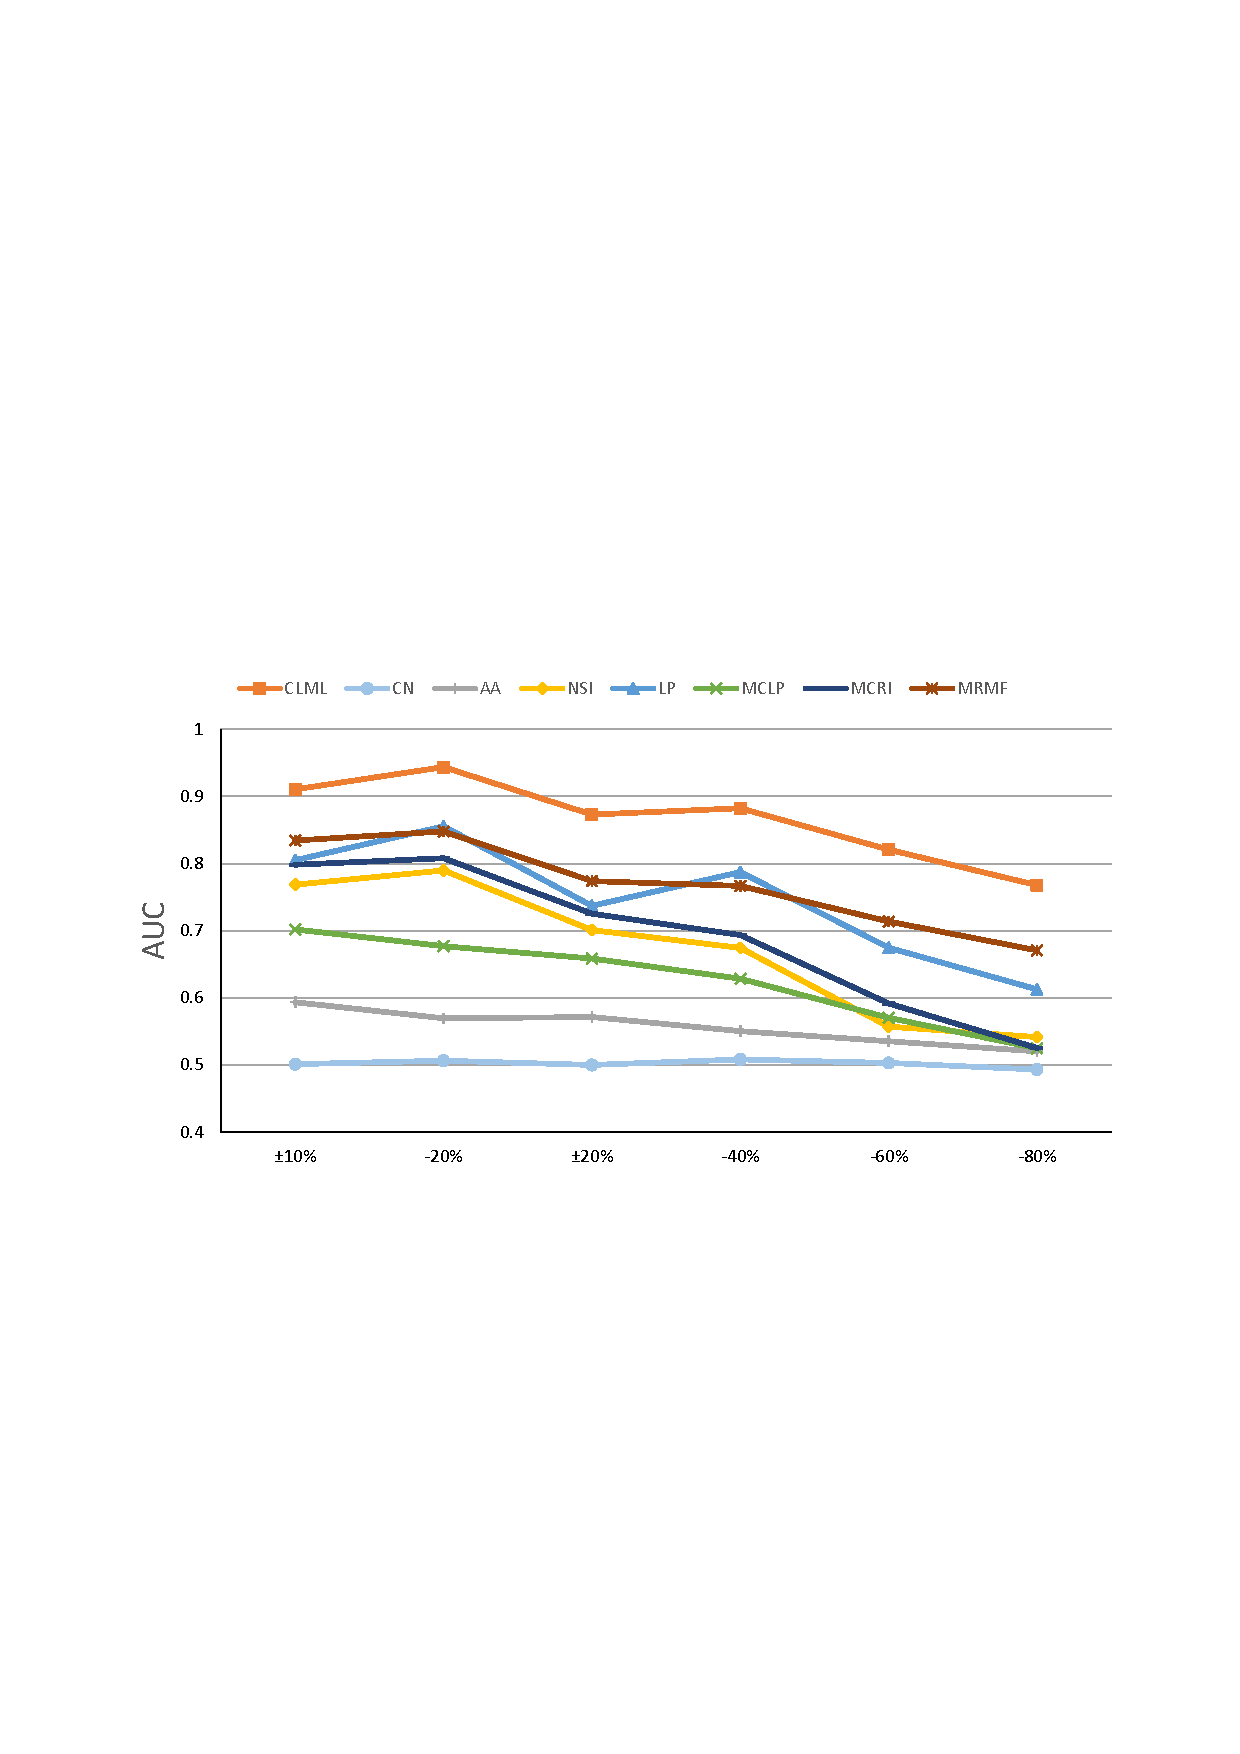
\includegraphics[width=0.45\linewidth]{AUC_NIPS.pdf}
    }
    \caption{各算法在不同数据集上的鲁棒性实验}
    \label{experiments:fig:robust}
\end{figure}


从图\ref{experiments:fig:robust}中可以看出:
第一,所有算法的性能都会随着数据的缺失而有不同程度的下降,在数据仅剩20\%时AUC值最低;
第二,CLML的AUC曲线相对平缓,即下降速率相对缓慢,并且始终高于其它算法。
综上所述,我们可以说CLML算法的鲁棒性要优于其它算法。

\subsection{节点度数与算法性能的关系}
从图\ref{experiments:fig:robust}中我们还可看出,虽然CLML在各个数据集上的预测结果都优于其它算法,
但它本身在不同数据集上的预测结果仍有一定变化,因此我们希望知道数据结构特点和预测效果的关系。


在对式(\ref{method:formula:self_repre})的推导过程中提到,需要让空间中的每一个点(即D或T矩阵中的每一个元素)都将其用空间中的其余所有点线性表出,
且距该点距离越近的点权重越大,越远的点权重越小,而度数越高的点又拥有更多的近邻点。
由此产生一个问题,节点的度数会对预测准确率产生影响吗?是否度数越高的点,与其相关的预测准确率越高呢?


\ref{experiments:sec:db_cv}节中已经统计了数据集中具有不同度的节点数量,我们将对具有不同度的节点分别进行预测,
对于预测后数据中的每个点,设与点发生关联的概率最大的前五个点的集合为,
置与中每个点产生关联的概率为1,与其余点的概率置为0后便得到了一个0-1矩阵;这之后,将新构造出的矩阵与原矩阵对比,
若点与中的任一点在原矩阵中的关联概率仍为1则便认为对点预测成功,否则预测失败;
最后,设具有不同度的集合中的预测准确率为预测成功的点占集合的比例,作为最终结果。
实验的关键代码见代码3.2:



\begin{lstlisting}[caption={节点度数与算法性能的关系实验代码},language=Matlab]
    interaction = sum(D,2); %统计每个点的度

    [rows1,~] = find(interaction == 1);
    [rows2,~] = find(interaction == 2);
    ...
    [rows10up, ~] = find(interaction > 80);
    .... %其余实验设置
    % 开始预测
    predictData = abs(DualManifoldWithLowRank(R, trainData, 
    W1, T, W2, alphas(10), betas(1), gammas(10), maxIterator)); 
    predictData = predictData + predictData';

    [~, index] = sort(predictData, 1, 'descend');
    index = index(1:5,:); %选出前五个最可能发生关联的点
    count = 1;
    for i = 1 : samp_amount
    if(sum(D(index(:,i),i)) > 0) 
    % 若两集合有交集,则记录下当前的点
        results(count,1) = i;
        count = count+1;
    end
        
    end
    %统计成功预测出的不同度的点
    [result1,~,~] = intersect(results,rows1); 
    [result2,~,~] = intersect(results,rows2);
    ...
    [result10up,~,~] = intersect(results,rows10up);

    a1 = length(result1) / length(rows1); %预测准确率
    ...
    a7 = length(result10up) / length(rows10up);

\end{lstlisting}


因为节点数量会随着其度数增大而减少,为了实验稳定性,我们在度数大于5后对节点分段划分来做对比,
图\ref{experiments:fig:degree_auc}为初步实验的结果,其中横轴代表节点的度数,纵轴代表算法在每类节点上的预测准确率值。
从图\ref{experiments:fig:degree_auc}中可以看出,无论哪个数据集,预测准确率在具有更高度数的节点上的确会有所提升,这一点在DouBan数据集上尤为突出:
其准确率在度为1的节点中仅为0.5左右,几乎等于随机分类器的准确率;
但随着节点度数的上升,准确率有明显的提升直至最后稳定值0.88上下。


\begin{figure}
    \centering
    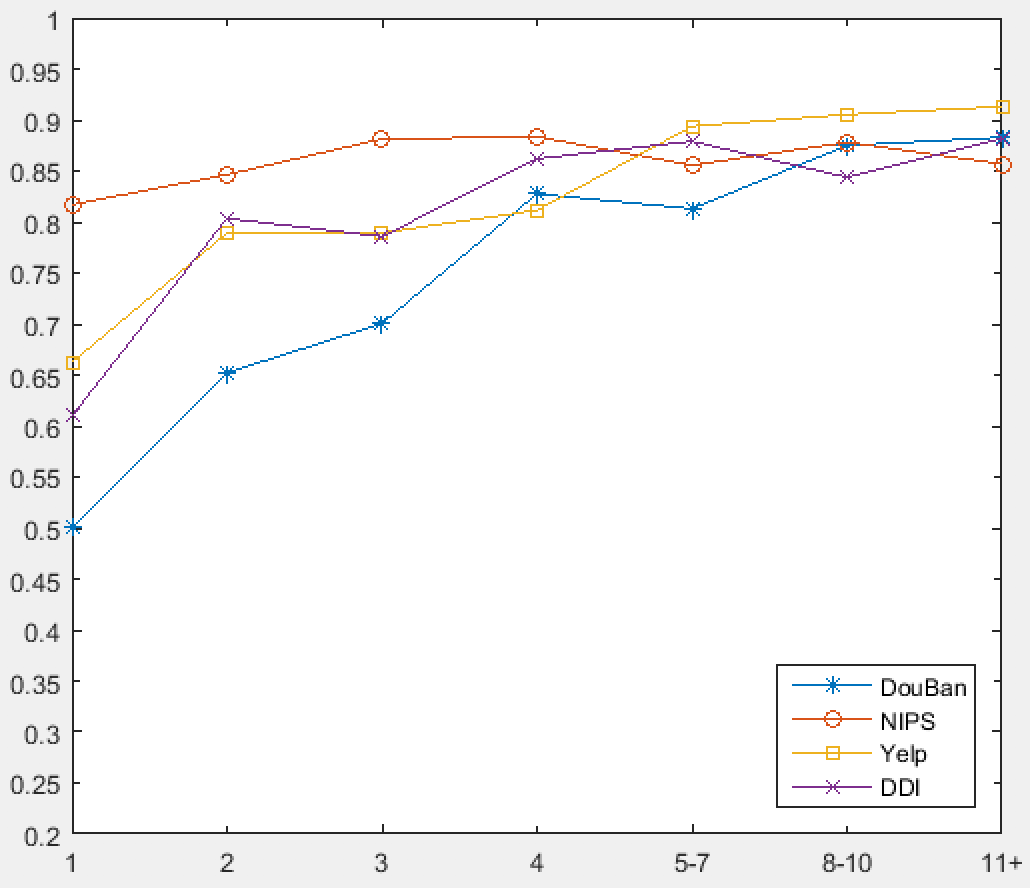
\includegraphics[width=0.6\linewidth]{degree_auc.png}
    \caption{节点度数和准确率的关系}
    \label{experiments:fig:degree_auc}
\end{figure}

但针对本次实验现象我们还存在一个疑问:
图\ref{experiments:fig:degree_auc}显示度数少的节点有非常多,而实验仅从中选取了少部分节点,而对于度数高的节点,因其数量很少故实验时使用了全部的数据,
那么曲线的上升是否是因为使用的训练数据比例提升了而不是因为节点的度数提升了呢?
为此我们针对Douban、Yelp这两个有较多低度数节点(因此训练数据比例也更低)的数据集做了进一步实验。


\begin{figure}
    \centering
    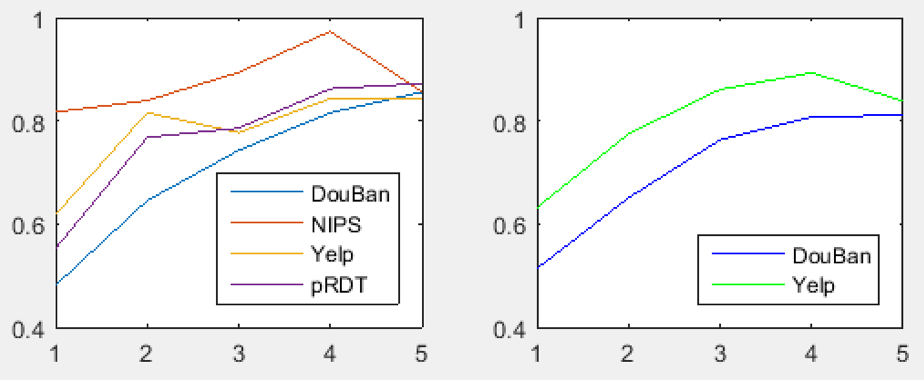
\includegraphics[width=0.85\linewidth]{degree_auc2.png}
    \caption{扩大对低度数节点的采样比例后的实验结果对比}
    \label{experiments:fig:degree_auc2}
\end{figure}

我们扩大了对低度数节点的抽取比例,若该做法可使算法对低度数节点的预测准确率有明显提升,
则我们可以认为图\ref{experiments:fig:degree_auc}中曲线的上升主要是由训练数据比例增大导致的,和节点度数无关。
提高了对度数为1、2、3的节点的抽取比例后得到的曲线(右)和原曲线(左)的对比如图\ref{experiments:fig:degree_auc2}。
从图中可看出,即使提高了部分节点的采样比例,曲线仍呈同样的上升趋势且在度数低的节点上的预测准确率并无显著变化,
因此我们可以对上述疑问作出否定回答,即预测准确率与采样比例并无明显关联。


\subsection{聚类系数与算法性能的关系}
在[12][13]中均提到,聚集程度较高的簇大部分情况下都获得更好的预测效果;
又因为聚集程度高的网络,其矩阵往往是低秩的,而CLML本身就假设了数据的低秩性并引入了低秩约束。
于是我们希望知道数据的聚集程度是否能直接影响到算法性能。
为此,我们在本次实验中使用了聚类系数来衡量矩阵的聚集程度,并观察算法对具有不同(全局)聚类系数的网络的预测结果是否会有差异。


全局聚类系数的计算基于节点三元组。三元组是由三个节点和两条链接(开放三元组)或三个节点和三条链接(闭合三元组)组成的,
设闭合三元组的个数为A,开放三元组的个数为B,则全局聚类系数为:
\begin{equation}
Clustering\ Coefficient=\frac{A}{B}
\end{equation}


实验时,我们随机从NIPS数据集中的$D$、$R$、$T$矩阵选取部分节点形成子集$D^{'}$,$R^{'}$,$T^{'}$,利用式(3.4)计算$D^{'}$的全局聚类系数$CC_{D^{'}}$,
再使用CLML在子集上做链接预测,计算此次预测的$AUC_{D^{'}}$便可得到一点$P_1(CC_{D^{'}}, AUC_{D^{'}})$;
重复上述过程N次便可得到$P_i(i=1,2,...N)$。图\ref{experiments:fig:cc_auc}展示了本次实验的结果,从中可大致看出当集合的聚类系数越高,模型在其上的AUC越高。


\begin{figure}
    \centering
    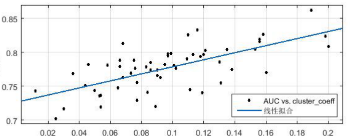
\includegraphics{CC_auc.png}
    \caption{CLML在具有不同聚类系数的数据集下预测时的AUC值}
    \label{experiments:fig:cc_auc}
\end{figure}


\subsection{案例分析}
在先前的实验中,我们在阐释CLML算法在各数据集上的结果时仅给出了如AUC、AUPR值这样抽象的数学结论。
而这一节为了进一步具体地看出CLML在实际应用中的价值,我们将CLML在做药物-药物关联预测时的结果从现实意义上做了分析,并将部分结果做了可视化处理。


在上文中提到,算法最终的结果是一个概率矩阵P,矩阵中的每个元素表示点i与点j产生关联的概率,在药物-药物关联预测中的意义即为药物i和药物j在临床使用时发生相互作用的概率。
为了验证CLML的实际意义,我们从预测结果中选取了前十个有着最大概率且未在Drugbank中收录的链接(相互作用),
并从Drugbank中找到了其对应的药物名称,如表\ref{experiments:table:case_study}所示。
在表中加粗的行表示其代表的相互作用已在其它论文、数据库或权威信息源得到了验证,
这些也可从Interaction Checker tool网站中检索到。
在这10个潜在关联中,有8个(80\%)已被验证为正确,这足以证明CLML算法在药物-药物关联预测这类实际应用场景下的有效性。
图\ref{experiments:fig:network}以表中所涉及的药物为例画出了与其相关的所有药物间的关系网络,节点颜色表示其度数,颜色越深则其度数越高;
方形节点为表\ref{experiments:table:case_study}中涉及到的药物,粗实线表示预测出且被验证为存在的关联,粗虚线表示预测出但尚未得到验证的关联


举例来说,在概述中提到,患有抑郁症等情绪障碍的患者需要长期服用抗抑郁类药物,而此类患者又往往伴随其它病灶,需要同时服用多种药物,因此导致抗抑郁类药物成为发生DDI的“主力军”。
在表\ref{experiments:table:case_study}的第七行中,我们预测出了一例由帕罗西丁(Paroxetine)与盐酸多奈哌齐(Donepezil)共同临床使用引起的相互作用,
其中前者就是一类被称为SSRIs的抗抑郁药物,在看到其临床效果之前可能需要数周的治疗,它和盐酸多奈哌齐会互相影响(抑制或促进都有可能)彼此的药物代谢作用从而影响到药效,
因此被建议临床使用时需有医生监控。


\begin{center}
    \tablecaption{预测出的前十名最有可能发生的DDI}
    \begin{tabular}{c|c|c}\hline
    概率排名 & DrugBank ID & 药品名称\\ \hline
    \bfseries 1 & \bfseries DB00777, DB00674 & \bfseries Propiomazine, Galantamin \\
    \bfseries 2 & \bfseries DB01238, DB00674 & \bfseries Aripiprazole, Galantamine \\
    \bfseries 3 & \bfseries DB00777, DB00843 & \bfseries Propiomazine, Donepezil \\
    4 & DB00715, DB00382 & Paroxetine, Tacrine \\
    \bfseries 5 & \bfseries DB00777, DB00382 & \bfseries Propiomazine, Tacrine \\
    \bfseries 6 & \bfseries DB01238, DB00843 & \bfseries Aripiprazole, Donepezil \\
    \bfseries 7 & \bfseries DB00715, DB00843 & \bfseries Paroxetine, Donepezil \\
    \bfseries 8 & \bfseries DB01238, DB00726 & \bfseries Aripiprazole, Trimipramine \\
    9 & DB00382, DB01239 & Tacrine, Chlorprothixene \\
    \bfseries 10 & \bfseries DB00382, DB00420 & \bfseries Tacrine, Promazine \\ \hline
    \end{tabular}
    \label{experiments:table:case_study}
\end{center}


\begin{figure}
    \centering
    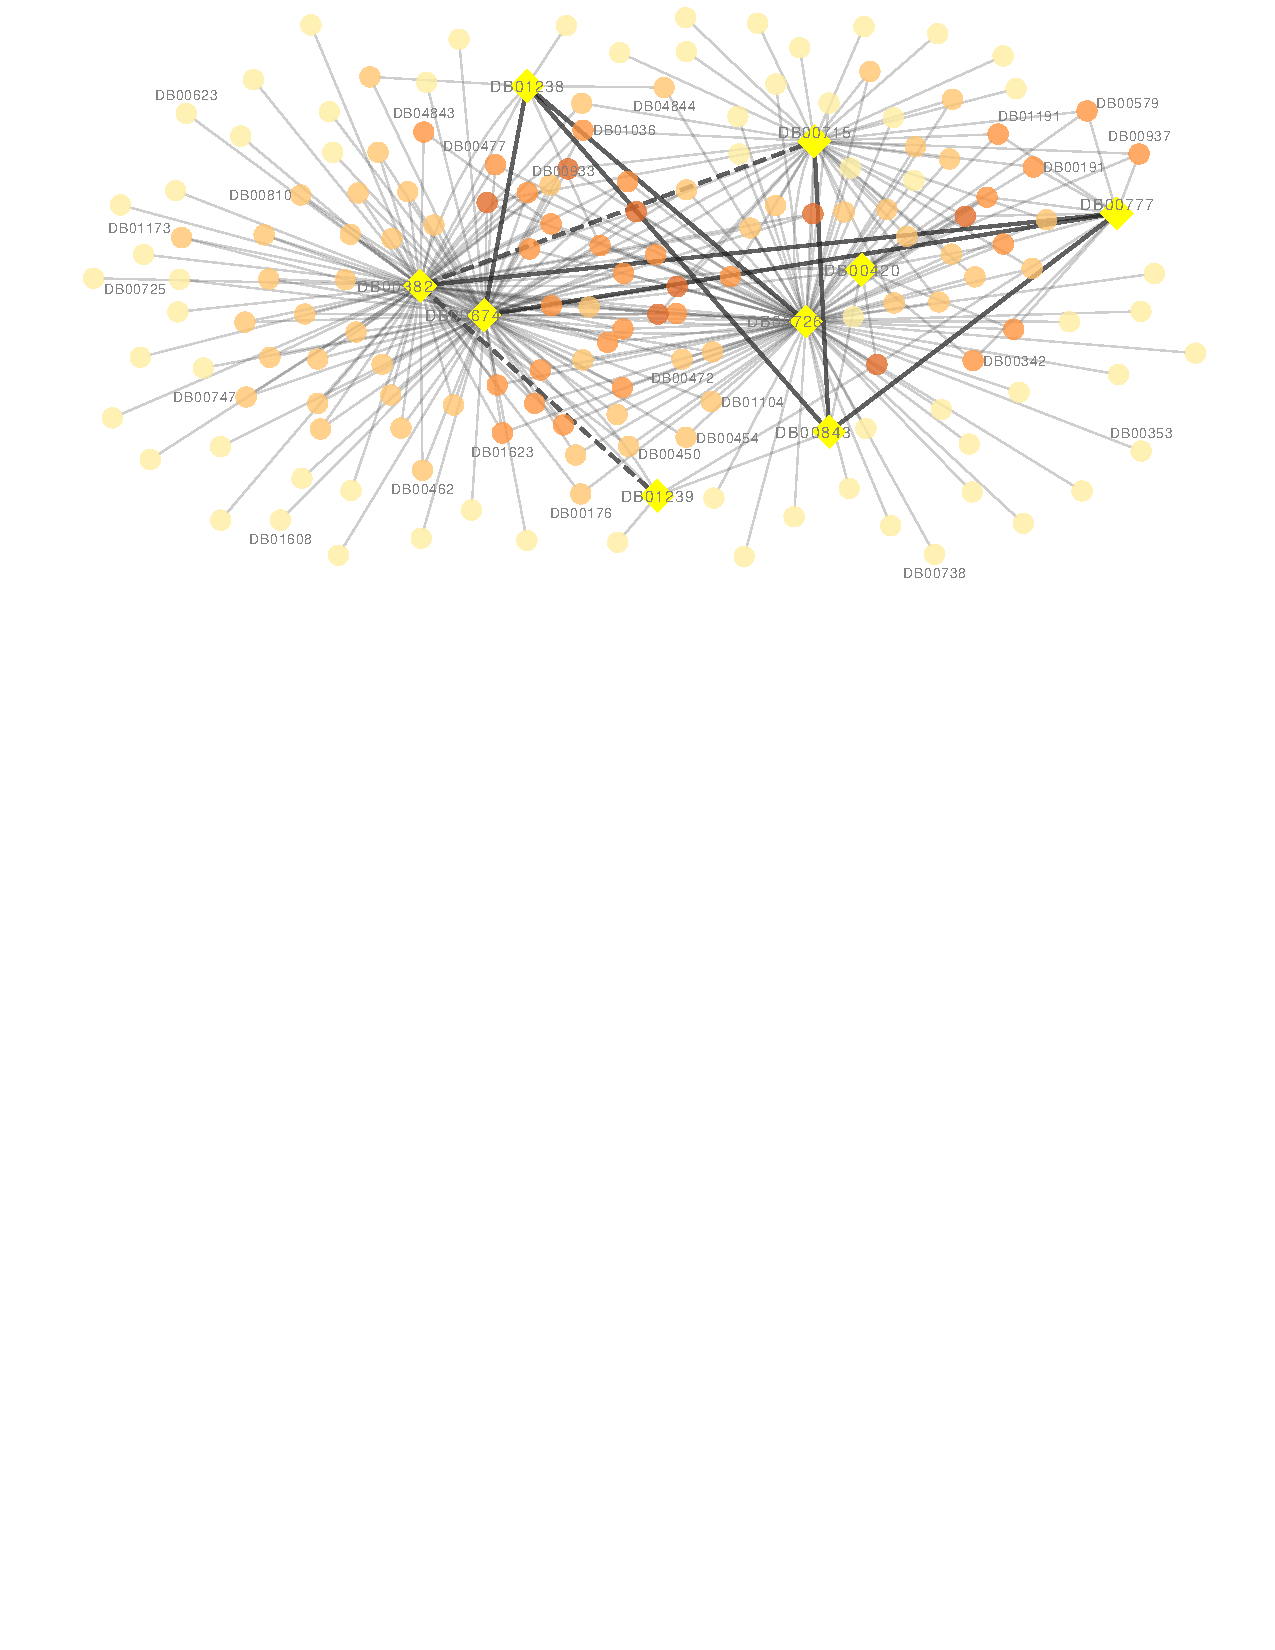
\includegraphics[width=0.95\linewidth]{network.pdf}
    \caption{药物互作网络的可视化图}
    \label{experiments:fig:network}    
\end{figure}


\section{本章小节}
在这一章中我们通过实验得到了CLML算法的各项性能,
其中通过实验一我们得到了CLML和其它比较算法在各个数据集上的AUC、AUPR等性能指标,并进一步用后续检验得出了CLML优于其它算法的结论;
通过实验二我们发现CLML较其它算法而言具有更好的鲁棒性;
实验三告诉我们,CLML在越密集的点(即度数越大的点)上预测准确率越高;
实验四在上一个实验的基础上又检验了数据集本身的聚集程度和准确率的关系,得出算法在聚集程度越高的数据集上预测效果越好的结论;
实验五将CLML实际应用到了药物-药物关联预测上,从现实意义上分析了实验结果并将结果做了可视化。
综合以上各个实验的结论后我们可以看出,CLML算法从整体性能上就要优于其它对比算法,且在实际问题中依然很有效率。
